\subsection{\swin}
\label{subsec:swin}

\swin{} adalah sebuah arsitektur \vitfull{} yang dirancang sebagai penopang dalam berbagai tugas \cv{} seperti klasifikasi gambar, deteksi objek, dan segmentasi semantik. Nama "Swin" berasal dari konsep
"\emph{Shifted Window}" yang menjadi elemen utama dalam desainnya. Tidak seperti \vit{} yang menggunakan metode \selfattention{} secara global
pada seluruh gambar, \swin{} memperkenalkan \selfattention{} berbasis \emph{local window} yang secara signifikan mengurangi kompleksitas komputasi \parencite{liu2021swin}. Perbedaan pendekatan \swin{} dan \vit{} dapat dilihat pada \autoref{fig:Swin-vs-ViT}. 

\autoref{fig:Swin-shifted-window} menujukkan pendekatan \shiftedwindow{} pada \swin. Selain itu, \swin{} mengadopsi arsitektur hierarkis yang mirip dengan \cnn. Arsitektur ini memungkinkan ekstraksi fitur pada berbagai skala dan menjadikannya lebih efisien untuk menangani gambar resolusi tinggi dan berbagai prediksi.

\begin{figure}[htbp]
    \centering
    
\includegraphics[width=0.7\textwidth]{images/swin-vit.png}
    \caption{Perbandingan antara \swin{} dan \vitfull{} \parencite{liu2021swin}.}
    \label{fig:Swin-vs-ViT}
\end{figure}

\begin{figure}[htbp]
    \centering
    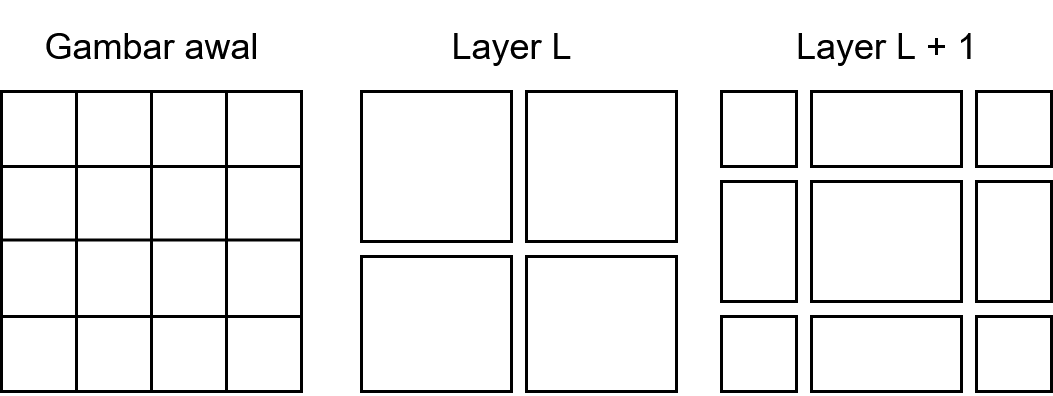
\includegraphics[width=0.7\textwidth]{images/swin-shifted-window.png}
    \caption{Pendekatan \shiftedwindow{} pada \swin{} \parencite{liu2021swin}.}
    \label{fig:Swin-shifted-window}
\end{figure}

Pada \swin, terdapat empat tahap. Pada setiap tahap, resolusi fitur akan secara bertahap dikurangi saat melalui lapisan \emph{patch merging} seperti pada \autoref{fig:swin-architecture}. Contohnya pada tahap satu, resolusi gambar $\frac{H}{4} \times \frac{W}{4}$ dengan dimensi fitur awal C. Kemudian pada tahap dua, resolusi dikurangi menjadi $\frac{H}{8} \times \frac{W}{8}$ dan 
dimensi fitur dinaikkan menjadi 2C. Tahap ini akan berlanjut hingga pada tahap empat dengan resolusi $\frac{H}{32} \times \frac{W}{32}$ dan dimensi 8C. Dengan struktur ini, \swin{} mampu menangkap informasi pada berbagai skala, seperti fitur lokal 
dan global, yang sangat penting dalam \emph{computer vision} seperti \emph{object detection}. 

\autoref{fig:swin-architecture} menunjukkan arsitektur dan cara kerja \swin. Gambar yang masuk dengan dimensi $H \times W$ akan dikonversi menjadi beberapa patch atau potongan kecil $4 \times 4$ pixel. Setiap \patch{} ini kemudian dianggap sebagai token, dan fitur awalnya direpresentasikan oleh nilai RGB-nya. Fitur ini kemudian 
diproyeksikan ke dimensi tertentu C melalui lapisan \emph{embedding} linier seperti yang ditunjukkan pada \autoref{fig:swin-architecture}.

\begin{figure}[htbp]
    \centering
    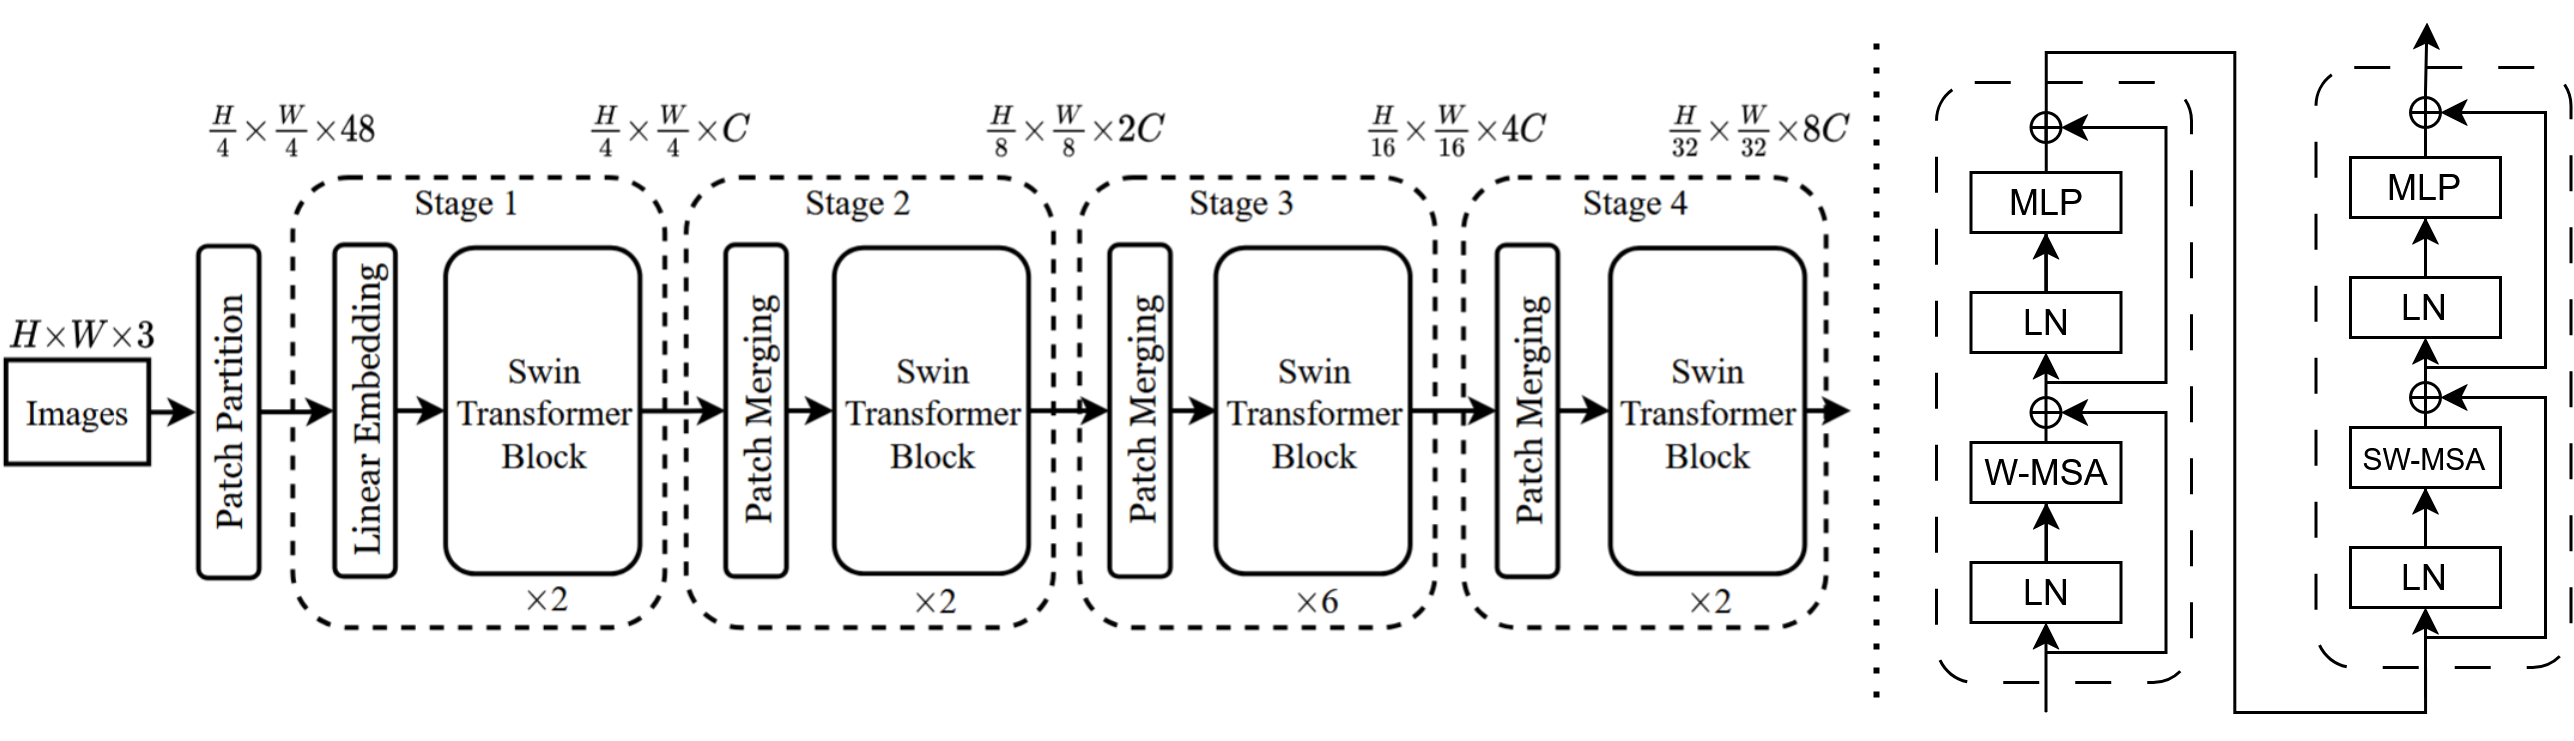
\includegraphics[width=1\textwidth]{images/swin-architecture.png}
    \caption{Arsitektur dan cara kerja \swin{} \parencite{liu2021swin}.}
    \label{fig:swin-architecture}
\end{figure}

\swin{} menggunakan \emph{Window Multi-Head Self-Attention} (W-MSA). Dengan metode ini, mekanisme \selfattention{} hanya dilakukan dalam \emph{window} lokal yang \emph{non-overlapping}. Contohnya ditunjukkan pada \autoref{fig:Swin-shifted-window}. 
Setiap \emph{window} memiliki ukuran $M \times M$ (umumnya $7 \times 7$) dan dengan membatasi \emph{attention} pada setiap \emph{window}, kompleksitas komputasi berkurang dari kuadratik menjadi linear.

Untuk memungkinkan koneksi \emph{cross-window}, \swin{} 
menggunakan metode \emph{Shifted Window Multi-Head Self-Attention} (SW-MSA). 
Dalam metode ini, setiap window akan bergeser pada lapisan berikutnya dengan jarak tertentu (misalnya setengah ukuran jendela). Ini menciptakan koneksi \emph{cross window} tanpa menambah banyak beban komputasi. Proses ini dapat dilihat pada \autoref{fig:Swin-shifted-window}. Window pada lapisan $l$ dan $l+1$ digeser untuk menciptakan interaksi 
satu sama lain. Dalam proses \emph{self-attention}, Swin Transformer menggunakan \textit{relative position bias} untuk menangkap hubungan spasial antar \patch.
